%background
\chapter{Background and Definition} 

%\label{ch:bg}
In this chapter, we will introduce some background of the algorithm and theory, which we used in the following research and proof. This part includes: benefit of randomized algorithm in game tree evaluation, minimax principle, Nor-tree definition and proof of its equivalence with AND-OR tree, Nor-tree evaluation process, reluctant input, which are all important in our research.


\section{Background}
\subsection{Benefit of Randomized Algorithm}
In previous chapter, we showed that randomized algorithm will have better expected number in evaluating compared with deterministic algorithm in some situation. We will prove this by induction. For an AND-OR tree $T$ with height $2k$(denoted as $T_{2k}$), the expected number for deterministic algorithm is $4^k$, now we argue that for the randomized algorithm we mentioned before the expected cost is at most $3^k$.

The basis condition when $k = 1$ just follows the analysis we made in chapter 1. Then we assume that for $T_{2k-1}$ the expected number needs to be read is $3^{k-1}$. Then by induction, we firstly analyze a tree with an AND node as root. If the root evaluates to 1, then both of its children at OR node return 1. The expected cost of this situation is $2 \times 3^{k-1}$, because both of the children need to be evaluated. On opposite, if the root evaluates to 0, the with probability $\frac{1}{2}$ the $0$ node will be choose first, then the expected cost is $\frac{1}{2} \times 3^{k-1}$. Other side, with $\frac{1}{2}$ probability the 0 one will be visit in second step, then $2\times \frac{1}{2} \times 3^{k-1}$. Then putting these two result together, we could determine the expected cost of this AND-OR tree is
\begin{equation}
	\frac{1}{2} \times 3^{k-1}+2\times \frac{1}{2} \times 3^{k-1}=\frac{3^k}{2}
\end{equation}
Similarly, we could also get root node is an OR node has the same expected cost. Therefore we could see that randomized algorithm is better than deterministic algorithm in game tree evaluating.  

\subsection{Minimax Principle}
Minimax Algorithm is widely used in decision making and game theory in order to find the optimal move for a specific player. The minimax principle is the only known general technique for proving lower bounds of randomized algorithms. It only could be applied to algorithms those could finish in finite time. In minimax algorithm, we assuming that both the player and his opponent play optimally. There is an example for illustrating the basic method of it:

\begin{figure}[H]
	\centering
	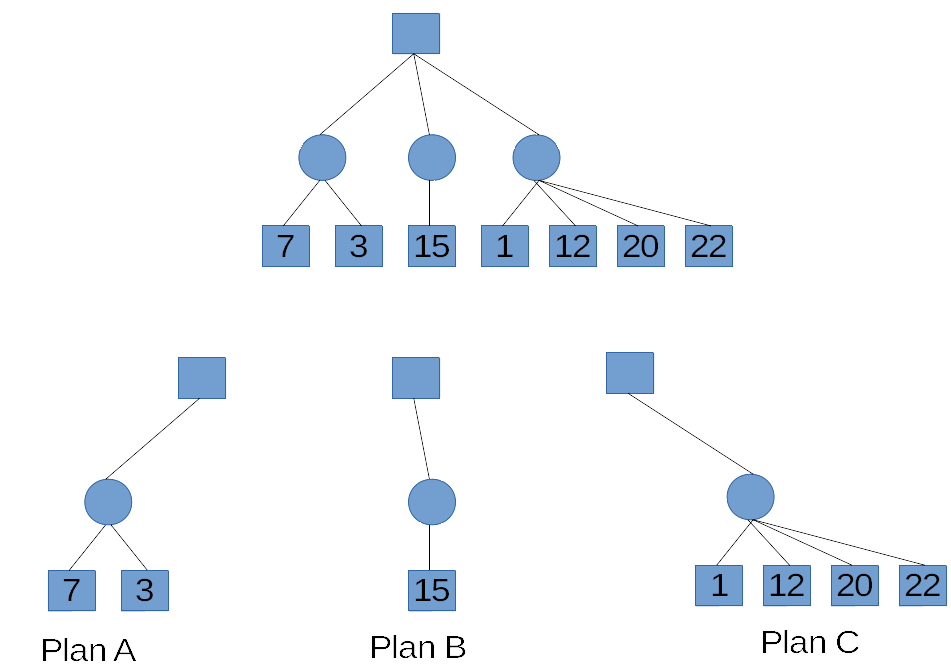
\includegraphics[width=0.5\linewidth]{minimax0}
	\caption{example of minimax principle}
	\label{fig:minimax0}
\end{figure}
Let square be player A ,and circle representing player B. Each leaf represents a possible benefit for player A. The aim of this game is for B to minimize A's benefit and A will try to maximize his benefit. If player A choose Plan A, then player B has two choices, in order to minimize player A's benefit. B will choose 3. For Plan B, player B has no choices but to let player A get 15. At last if plan C is chosen, then  player A could only get 1 benefit. Therefore in order to maximize his benefit, player A will choose plan B.

In order to understand the minimax principle theoretically. We will introduce some basic concept in game theory. One important concept is two-person zero-sum game, in which minimax principle could be applied. Let's say there are two player T and F. They will choose from three tarot card: Fool, Justice, Judgement. They don't know what card the opposite choose. Then they will show the card at the same time. The winner is determined by the following rules: The Fool beats Justice and wins 5 dollar; Justice wins the Judgement and Judgement will beat the Fool. Both of this two cases wins 3 dollar.If they choose the same card, then it comes to a draw. The game described above os an instance of a two-person zero-sum game. A two-person zero-sum game always could be represented as a payoff matrix. Like the game above could be:
\begin{table}[H]
	\caption{Matrix for tarot game}
	\begin{tabular}{lccc}
		\hline
		\hline
		  T $\backslash$ F & Fool & Justice & Judgement \\
		  \hline
		  \hline
		  Fool & 0 & 5 & -3\\
		  \hline
		  Justice & -5 & 0 & 3\\
		  \hline
		  Judgement & 3 & -3 & 0\\
		 \hline
		 \hline
	\end{tabular}
\end{table}

Let's set the matrix as $M$. Every row could denote the strategy chosen by player T and every column could be the strategy for player F.Then the entry $M_{ij}$ is the amount paid from T to F when T chooses strategy $i$ and F chooses $j$. Therefore, F will try to minimize the payoff and T will try to maximize the payoff. Because both player T and F has no idea about what strategy their opponent will choose. If T choose strategy $i$, then the payoff will be $min_jM_{ij}$ and no matter what F will choose the payoff is guaranteed. We could see the optimal strategy for player T is to maximize $min_jM_{ij}$.Similarly, We could get the player F's optimal payoff is $min_jmax_iM_{ij}$. For all payoff matrices we have:
\begin{lemma}
	$max_imin_jM_{ij} \le min_jmax_iM_{ij}$
\end{lemma}  
When the equality exists, which mean the game is said has a solution and the value of the game is the equal to the lower bound of payoff from player trying to maximize it or the upper bound of payoff from player trying to minimize it. The solution also could be called as saddle point\cite{SA}. However, not all games have a solution under this type strategy. Like in tarot game, Value for T is 3 and F is -3. Both of the player will try to improve their payoff as much as possible. So far we discussed is about pure or deterministic strategy. In order to solve the game has no solutions, we should use strategies with randomization in it, which are called mixed or randomized strategies. A randomized strategy is a probability distribution on the set of all possible strategies. For example, in tarot game(Let's say payoff matrix $M$ has m rows and n columns), player T will have probability $p_i$ to choose row $i$ as his strategy and the randomized strategy for T is a vector $\vect{p} = (p_1,...,p_n)$. Similarly, let's define randomized strategy for F as $\vect{q} = (q_1,...,q_m)$, which denotes the probability distribution on columns. Therefore we could get the expectation payoff as:
$$ E[pay] = p^TMq = \sum_{i=1}^{n}\sum_{j=1}^{m}p_iM_ijq_j$$   
Similarly to how we analyze deterministic strategy, we could get The optimal lower bound for player T is $L = max_pmin_qp^TMq$ and optimal upper bound for player F is $U=min_qmax_pp^TMq$. Then here comes a well-known Minimax Theorem of von Neumann\cite{VON}.For any two-person zero-sum game specified by a payoff matrix M:
\begin{theorem}
	$max_{\vect{p}}min_{\vect{q}}\vect{p}^TM\vect{q} = min_{\vect{q}}max_{\vect{p}}\vect{p}^TM\vect{q}$
\end{theorem}
which means that this type of game always has a solution and a pair of randomized strategies ($\vect{p}$,$\vect{q}$), which helps reach the solution is the saddle point of the game. We also could easily find that $\vect{p}^TM\vect{q}$ is a linear function of $\vect{q}$ and it could be simplified by setting 1 to the smallest coefficient $q_j$ and 0 to others. We could find that if player F knows the probability distribution $\vect{p}$, then his optimal solution will be a deterministic strategy. The theorem 1 also could be lead to a simplified version which invented by Loomis\cite{LOOMIS}:
\begin{theorem}
		$max_{\vect{p}}min_{j}\vect{p}^TMu_j = min_{\vect{q}}max_{i}e_{i}^{T}M\vect{q}$ (where $u_i$ means a unit vector with a 1 in i position and 0s in others)
\end{theorem}
\subsection{Yao's Principle}
Yao's principle, which also called 'minimax principle' claims that the expected cost of randomized algorithm on the worst-case input is no better than the expected cost for a worst-case probability distribution on the inputs of the deterministic algorithm that performs best against that distribution.\cite{YAO} Let's use the tarot game in previous game to illustrate this. We set player F as the one who apply the algorithm(every column), and player T as adversary choose the input(every row).Let's say the payoff from player F to player T is the valuable cost of the performance of an algorithm with rows as a finite set of all possible inputs and columns as a finite set of possible deterministic algorithms that always produces a correct solution. Clearly, player F will choose an algorithm which minimizes the payoff, and the  player T will try to maximize it.

In this problem, we could observe that the number of distinct inputs is equal to the number of distinct deterministic algorithms which could promise finish with correct solution. A deterministic strategy for player T is an input and for player F is a deterministic algorithm. A randomized strategy for T is a distribution over all inputs and a randomized strategy for F is a distribution over the space of deterministic algorithms\cite{M}. We could see this is a Las Vegas randomized algorithm\cite{LAS}. Let's set $L_F$ is the worst case algorithm cost for all deterministic algorithm and $U_T$ is the best case algorithm cost for the worst deterministic algorithm choice. We denote $L_F$ as the deterministic complexity for the game and $U_T$ as the randomized complexity \cite{S}. In this thesis, we will focus on complexity which is the expected algorithm cost of the best deterministic algorithm with worst distribution on input\cite{MT}. This  complexity is smaller than deterministic one because the algorithm knows the distribution.\cite{YAOC}

From Loomis Minimax Principle, we could get the complexity equals the least possible costs with any randomized algorithm. Now we could apply the Minimax Principle as:
Let $G$ be a two-person zero-sum game problem. It has a finite set $\vect{I}$ as input and a finite set $\vect{D}$ as the set of all possible, always correct deterministic algorithms. For instance I $\in \vect{I}$ and D $\in \vect{D}$, we denote C(I,D) as the cost for deterministic algorithm over input I. The probability distributions on $\vect{I}$ and $\vect{D}$ are $\vect{p}$ and $\vect{q}$. Then we could get theorem 1 and 2 as :
\begin{equation}
   max_{\vect{p}}min_{\vect{q}}E[C(\vect{I}_{\vect{p}},\vect{D}_{\vect{q}})] = min_{\vect{q}}max_{\vect{p}}E[C(\vect{I}_{\vect{p}},\vect{D}_{\vect{q}})]
\end{equation}

\begin{equation}
max_{\vect{p}}min_{D\in\vect{D}}E[C(\vect{I}_{\vect{p}},\vect{D})] = min_{\vect{q}}max_{I\in\vect{I}}E[C(I,\vect{D}_{\vect{q}})]
\end{equation}

Then the Yao's Minimax Principle comes:
\begin{theorem}
	$$min_{D\in\vect{D}}E[C(\vect{i}_{\vect{p}},D)] \le max_{I\in \vect{I}}E[C(I,\vect{D}_{\vect{q}})]$$
\end{theorem}

Yao's Principle is a very useful tool for proving the lower bound for randomized algorithm. It claims the expected cost of the optimal deterministic algorithm for a randomized chosen input distribution is the lower bound for the cost of optimal randomized algorithm for problem. The reduction to a lower bound on deterministic algorithms makes Yao's principle is very powerful in proving lower bound.\cite{YAOS}

\subsection{Nor-Tree Evaluation}
In previous chapter. We introduce the binary tree evaluation could be transformed to an AND-OR tree evaluation by limited the leaves value with in 0 and 1. In this thesis, we will use a more simplified tree model which called nor-tree, its logic is following:
\begin{figure}[H]
	\centering
	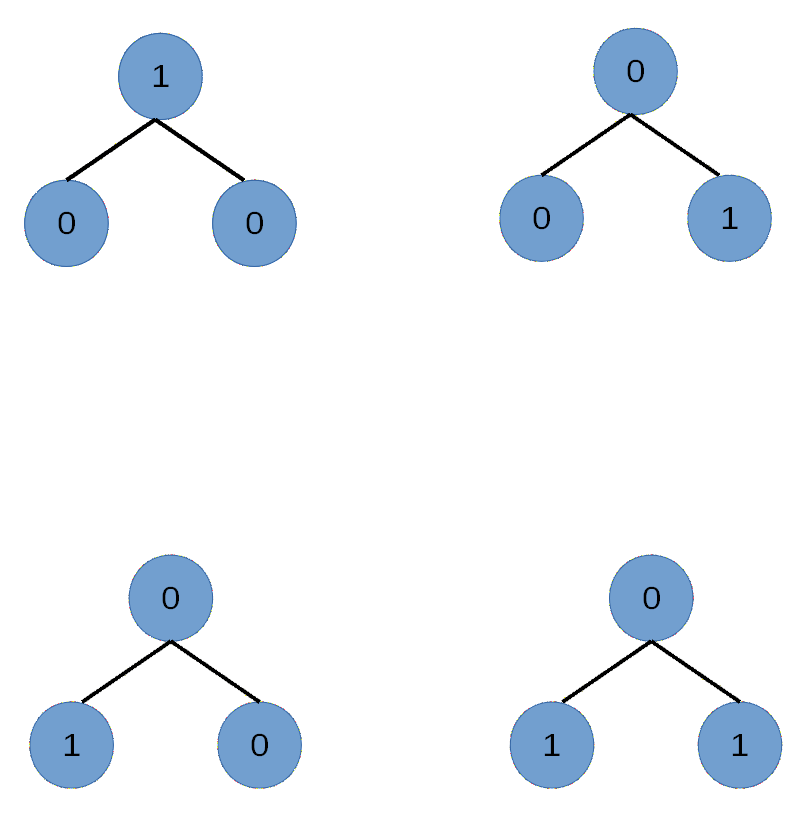
\includegraphics[width=0.5\linewidth]{Nortree}
	\caption{Nortree logic}
	\label{fig:nortree}
\end{figure}
A balanced binary tree whose all leaves are at the distance 2k from root is equal to the same structure nor-tree. Firstly, we already proved that this is equivalent to the same height AND-OR tree. Then Let's see when k = 1. Let's denote the 4 notes as a,b,c,d. The value of the root of AND-OR tree is $(a \bigvee b) \bigcap(c \bigvee d)$ and the nor-tree's is $\neg(a \bigvee b) \bigcap \neg (c \bigvee d)$. We could see this two is equal. Assuming that k=n-1 this claim is correct. Similarly, we could prove when k=n, this is also correct.
\begin{figure}[H]
	\centering
	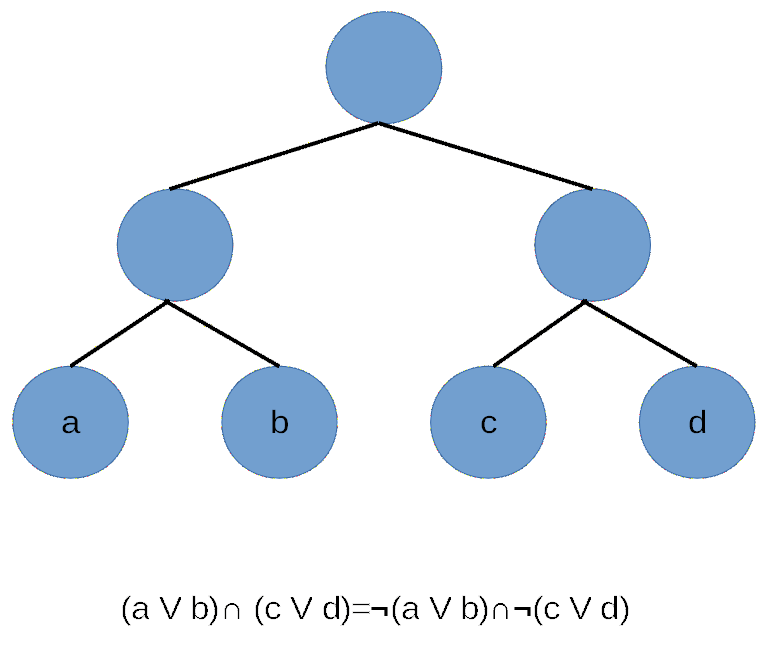
\includegraphics[width=0.5\linewidth]{ao_nor}
	\caption{AND/OR tree equivalent to Nor-tree with Same Height }
	\label{fig:aonor}
\end{figure}

Then for the evaluation of this nor-tree we have:
$$ h(x)=\left\{
\begin{aligned}
&h_{left}(x_L) + h_{right}(x_R) & if\ algorithm=L\ and\ left\ equals\ to\ 0\\
&h_{left}(x_L)  & if\ algorithm=L\ and\  left\ equals\ to\ 1\\
&h_{left}(x_L) + h_{right}(x_R) & if\ algorithm=R\ and\ right\ equals\ to\ 0\\
&h_{right}(x_R) & if\ algorithm=R\ and\ right\ equals\ to\ 1
\end{aligned}
\right.
$$
which could be described as:
\begin{lstlisting}[title=evaluation of nor-tree, frame=shadowboc]
1:NorEvaluation(node)
2:if (node.type = "LEAF") then
3:   return(node.value)
4:end if
5:if (node.type = "Nor") then
6:  Toss a coin
7:  if (Heads) then
8:  p1 = NorEvaluation(node.left)
9:  if(p1 = 1) then 
10:   return 0
11:  else
12:  p2= NorEvaluation(node.right) 	
13:    if(p2 = 0)
14:      return 1
15:    else
16:      return 0;
17:    end if
18:  end if
19:end if
\end{lstlisting}
Yao's principle has its flexibility in the choice of input distribution. In "Randomized Algorithm", the author just choose the distribution by arbitrary and ignored conditional probability in internal nodes. By experiments simulates the leaves value distribution with algorithm we find that the algorithm does not effect the best payoff of the tree, and we could find the pattern of the optimal nor-tree is:
\begin{enumerate}
	\item The value of the root is always 1.
	\item When the value of node equals to 0, the value of two leaves will has 1/2 probability to be (0,1) and 1/2 to be (1,0);
\end{enumerate}

In this thesis, we will use L(k,i) to denote the min expected leaves visited by algorithm of node 
in k level whose value is i(payoff for a tree of height k, its value is i, and k is even).

\section{Definitions}
We define the value of a leaf as its input value (leaf label), and 
the value of an internal node as true if both children are false,
and false otherwise.
We define
 an algorithm for a NOR tree $T$ as a process to find a specific ordering $\sigma$ of 
$T$'s leaves. It always starts with a leaves ordering. Based on the value of the vertices's already been determined, it will rearrange the ordering in order to determine the root's value by visiting as less leaves as possible. 

The prefix of $\sigma$ of length $t$ will be denoted as $\sigma_t$.
Given a leaf labeling and an ordering $\sigma$, 
we associate a logical time-stamp to each tree vertex as follows.
We will say that a leaf $u$ is evaluated at time $t$ 
if $\sigma_t$ is the shortest prefix of $\sigma$ containing $u$.
It is immediate to see that $u$ is evaluated at time $t$ if and only if
the $t$th element of $\sigma$ is $u$.
If $u$ is an internal node whose value is false,
we will say that $u$ is evaluated at time $t$ if 
$\sigma_t$ is the shortest prefix such that both children of $u$
have been evaluated at time $t$ or earlier. 
Conversely, if $u$ is an internal node whose value is true,
$u$ is evaluated at time $t$ if 
$\sigma_t$ is the shortest prefix such that at least one
child of $u$ whose value is false 
has been evaluated at time $t$ or earlier.
Intuitively, the definition captures the idea that the value of an 
internal node becomes available as soon as there is the minimum
amount of information needed to evaluate it. 
We define the  cost of a NOR tree algorithm
as the time at which the root is evaluated.
Note that once the root is evaluated, 
the remaining suffix of $\sigma$ is irrelevant to 
$\sigma$'s cost. 
In light of this observation, we will say that 
$\sigma$ omits leaf $u$ if leaf $u$ appears after
the root has been evaluated.
Similarly, we say that $\sigma'$ omits an internal node $x$ 
if node $x$ appears after the root has been determined.

Note that any tree traversal implicitly defines a 
leaf ordering $\sigma$ as the subsequence of the traversal order
containing only the leaves. 
Conversely, given a leaf ordering $\sigma'$, we define its 
canonical traversal as the vertex ordering whose leaf 
subsequence is $\sigma'$,
where a true internal node $u$ appears at the earliest point after
both of its children, and
where a false internal node $u$ appears at the earliest point after
one of its true children.
It is immediate to see that the evaluation order of $\sigma$ can be 
reconstructed from its canonical traversal. 

\begin{figure}[H]
	\centering
	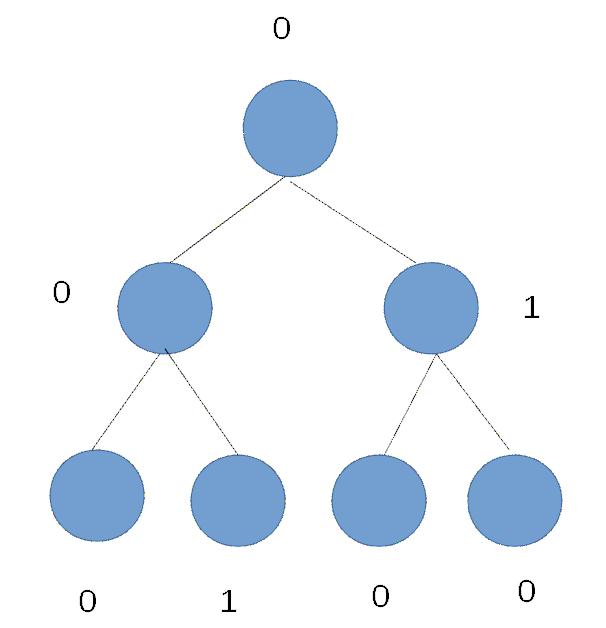
\includegraphics[width=0.3\linewidth]{def_0}
	\caption{A NOR-tree of height 2 with a binary labeling of the leaves
		and calculated values in the internal nodes.}
	\label{fig:def0}
\end{figure}
Figure \ref{fig:def0} shows an example of these definitions.
Suppose that an algorithm visits the four leaves from left to right.
Then, the corresponding leaf ordering is $\sigma' = (a, b, c, d)$.
The canonical ordering $\sigma$ can be constructed as follows.
First, since $\sigma'$ is a subsequence of $\sigma$, then
the leaves appear in the order $a, b, c, d$ within $\sigma$
Since $e$ is a false internal node, node $e$ appears in $\sigma'$
immediately after its true child $a$. 
Since $f$ is a true internal node, node $f$ appears in $\sigma'$ immediately
after $c$ and $d$. 
Finally, since $g$ is false, node $g$ appears in $\sigma'$ immediately
after $f$.
By putting these constraints together, we obtain that 
$\sigma' = (a, e, b, c, d, f, g)$.
It is immediate to see that a better algorithm would visit only three leaves
if $\sigma_3 = (a, c, d, b)$ and $\sigma'_3 = (a, e, c, d, f, g, b)$.
and that the optimal visit enables the tree evaluation by visiting
only the leaves $c$ and $d$ with 
$\sigma_2 = (c, d, a, b)$ and $\sigma'_2 = (c, d, f, g, a, e, b)$.
Note that the algorithm $\sigma_2$ omits the leaves $a$ and $b$.


%\bibliographystyle{plainnat}				%Uncomment this if you want a bibliography on each chapter
%\markright{\textit{Bibliography}}
%\renewcommand{\chaptername}{}
%\bibliography{my_references}

%\vfill

